% Introducing Dr.C: A Domain-Specialized Multi-Agent AI for Designing Csound Instruments and Plugins and Developing Educational, Generative and Audio Reactive Web Applications
% LAC 2026 Submission - Boulanger & Larrea

\def\papertitle{Introducing Dr.C: A Domain-Specialized Multi-Agent AI for Designing Csound Instruments and Plugins and Developing Educational, Generative and Audio Reactive Web Applications}
\def\paperauthorA{Richard Boulanger}
\def\paperauthorB{Mateo Larrea}

\documentclass[a4paper]{article}

\usepackage{LAC-26}
\usepackage[margin=2cm]{geometry}
\usepackage{amsmath,amssymb,amsfonts,amsthm}
\usepackage{euscript}
\usepackage[utf8]{inputenc}
\usepackage[T1]{fontenc}
\usepackage{ifpdf}
\usepackage{color}
\usepackage{listings}
\definecolor{mygrey}{rgb}{0.96,0.96,0.96}
\lstset{
  tabsize=4,
  basicstyle=\ttfamily\footnotesize,
  backgroundcolor=\color{mygrey},
  captionpos=b,
  breaklines=true
}

\usepackage[english]{babel}
\usepackage{caption}
\usepackage{subfig, color}

\setcounter{page}{1}
\ninept

\usepackage{times}

% pdf-tex settings: detect automatically if run by latex or pdflatex
\newif\ifpdf
\ifx\pdfoutput\relax
\else
   \ifcase\pdfoutput
      \pdffalse
   \else
      \pdftrue
\fi

\ifpdf % compiling with pdflatex
  \usepackage[pdftex,
    pdftitle={\papertitle},
    pdfauthor={\paperauthorA, \paperauthorB},
    colorlinks=false,
    bookmarksnumbered,
    pdfstartview=XYZ
  ]{hyperref}
  \pdfcompresslevel=9
  \usepackage[pdftex]{graphicx}
  \usepackage[figure,table]{hypcap}
\else % compiling with latex
  \usepackage[dvips]{epsfig,graphicx}
  \usepackage[dvips,
    colorlinks=false,
    bookmarksnumbered,
    pdfstartview=XYZ
  ]{hyperref}
  \usepackage[figure,table]{hypcap}
\fi

\title{\papertitle}

\twoaffiliations{
\paperauthorA}
{\href{https://www.berklee.edu}{Berklee College of Music} \\ Boston, MA, USA \\
{\tt \href{mailto:rboulanger@berklee.edu}{rboulanger@berklee.edu}}
}
{\paperauthorB}
{\href{https://ccrma.stanford.edu}{CCRMA, Stanford University} \\ Stanford, CA, USA \\
{\tt \href{mailto:mlarreaf@stanford.edu}{mlarreaf@stanford.edu}}
}

\begin{document}

\ifpdf
  \DeclareGraphicsExtensions{.png,.jpg,.pdf}
\else
  \DeclareGraphicsExtensions{.eps}
\fi

\maketitle

\begin{abstract}
We present Dr.C, an open-source AI system specialized for Csound that addresses fundamental limitations in general-purpose AI coding assistants. Dr.C implements a domain-specialized architecture combining multi-agent orchestration, curated knowledge retrieval, semantic validation, and an alternatives-first design paradigm that positions the AI as collaborator rather than autonomous generator. Key contributions include Csound-aware structural patching, contract validation beyond syntax checking, multi-tier knowledge retrieval, and design tree exploration. Dr.C is freely available under MIT license as a template for building domain-specialized AI assistants for FLOSS audio development.
\end{abstract}

\textbf{Keywords:} Csound, Domain-Specialized, Multi-Agent, Dr.C, Educational-Scaffolding

\section{Introduction}
\label{sec:intro}

Large language models (LLMs) like GPT-4 and Claude have enabled widespread adoption of AI-assisted programming. However, applying these general-purpose systems to computer music reveals limitations: syntax hallucination (Csound 6 vs. 7 incompatibilities), lack of curated domain knowledge, premature optimization, missing semantic validation, and poor educational scaffolding \cite{boulanger2000csound}. For Csound—a mature FLOSS audio language with 35+ years of evolution—these issues are acute, as LLMs trained on web-scraped code cannot navigate its significant version changes.

\subsection{Contributions}

We present \textbf{Dr.C}, a domain-specialized AI system for Csound development with the following contributions:

\begin{enumerate}
\item \textbf{Alternatives-first design paradigm:} A novel interaction model where the AI proposes 2--4 design alternatives varying by technique, character, and complexity before executing, keeping humans in creative control
\item \textbf{Multi-tier knowledge retrieval:} Combines opcode quick-reference cards, working example CSDs, prose from synthesis textbooks, and knowledge graph traversal with domain-aware query routing
\item \textbf{Semantic validation framework:} Beyond syntax checking—validates Cabbage widget bindings, parameter smoothing, UI layout, and user-defined locked parameters
\item \textbf{Multi-agent orchestration:} Specialized sub-agents for synthesis, effects, and modulation that execute concurrently on independent sub-tasks
\item \textbf{Session-based workspace isolation:} Safe experimentation with sandboxed temporary copies and explicit save/discard workflow
\item \textbf{Design tree exploration:} Non-linear version control capturing all explored alternatives with sonic characterization metadata
\end{enumerate}

Dr.C is intentionally scoped to Csound (.csd file) synthesis, Cabbage plugin development, and educational exploration—enabling deep specialization that outperforms general-purpose tools.

\section{System Architecture}
\label{sec:architecture}

\subsection{Multi-Agent System}

Dr.C implements a hierarchical multi-agent architecture with role-specific agents (Figure~\ref{fig:architecture}):

\textbf{Primary Agents:}
\begin{itemize}
\item \texttt{csound} (Claude Sonnet 4.5): Full-featured design agent with alternatives workflow and RAG
\item \texttt{csound-sine} (Claude Haiku 4.5): Lightweight fast-edit agent for quick fixes
\item \texttt{build}: General-purpose agent for non-Csound tasks
\end{itemize}

\textbf{Specialized Sub-Agents} (Claude Haiku 4.5 for cost/speed):
\begin{itemize}
\item \texttt{csound-synthesis}: Oscillators, FM/AM, additive/subtractive, physical modeling
\item \texttt{csound-effects}: Reverb, delay, filters, distortion, EQ, dynamics
\item \texttt{csound-modulation}: Envelopes, LFOs, control signals, MIDI/OSC
\end{itemize}

The permission system provides fine-grained control, denying all operations by default, allowing file reading and Csound tools, restricting edits to .csd files only, and prompting for access to external directories.

\begin{figure}[t]
\centerline{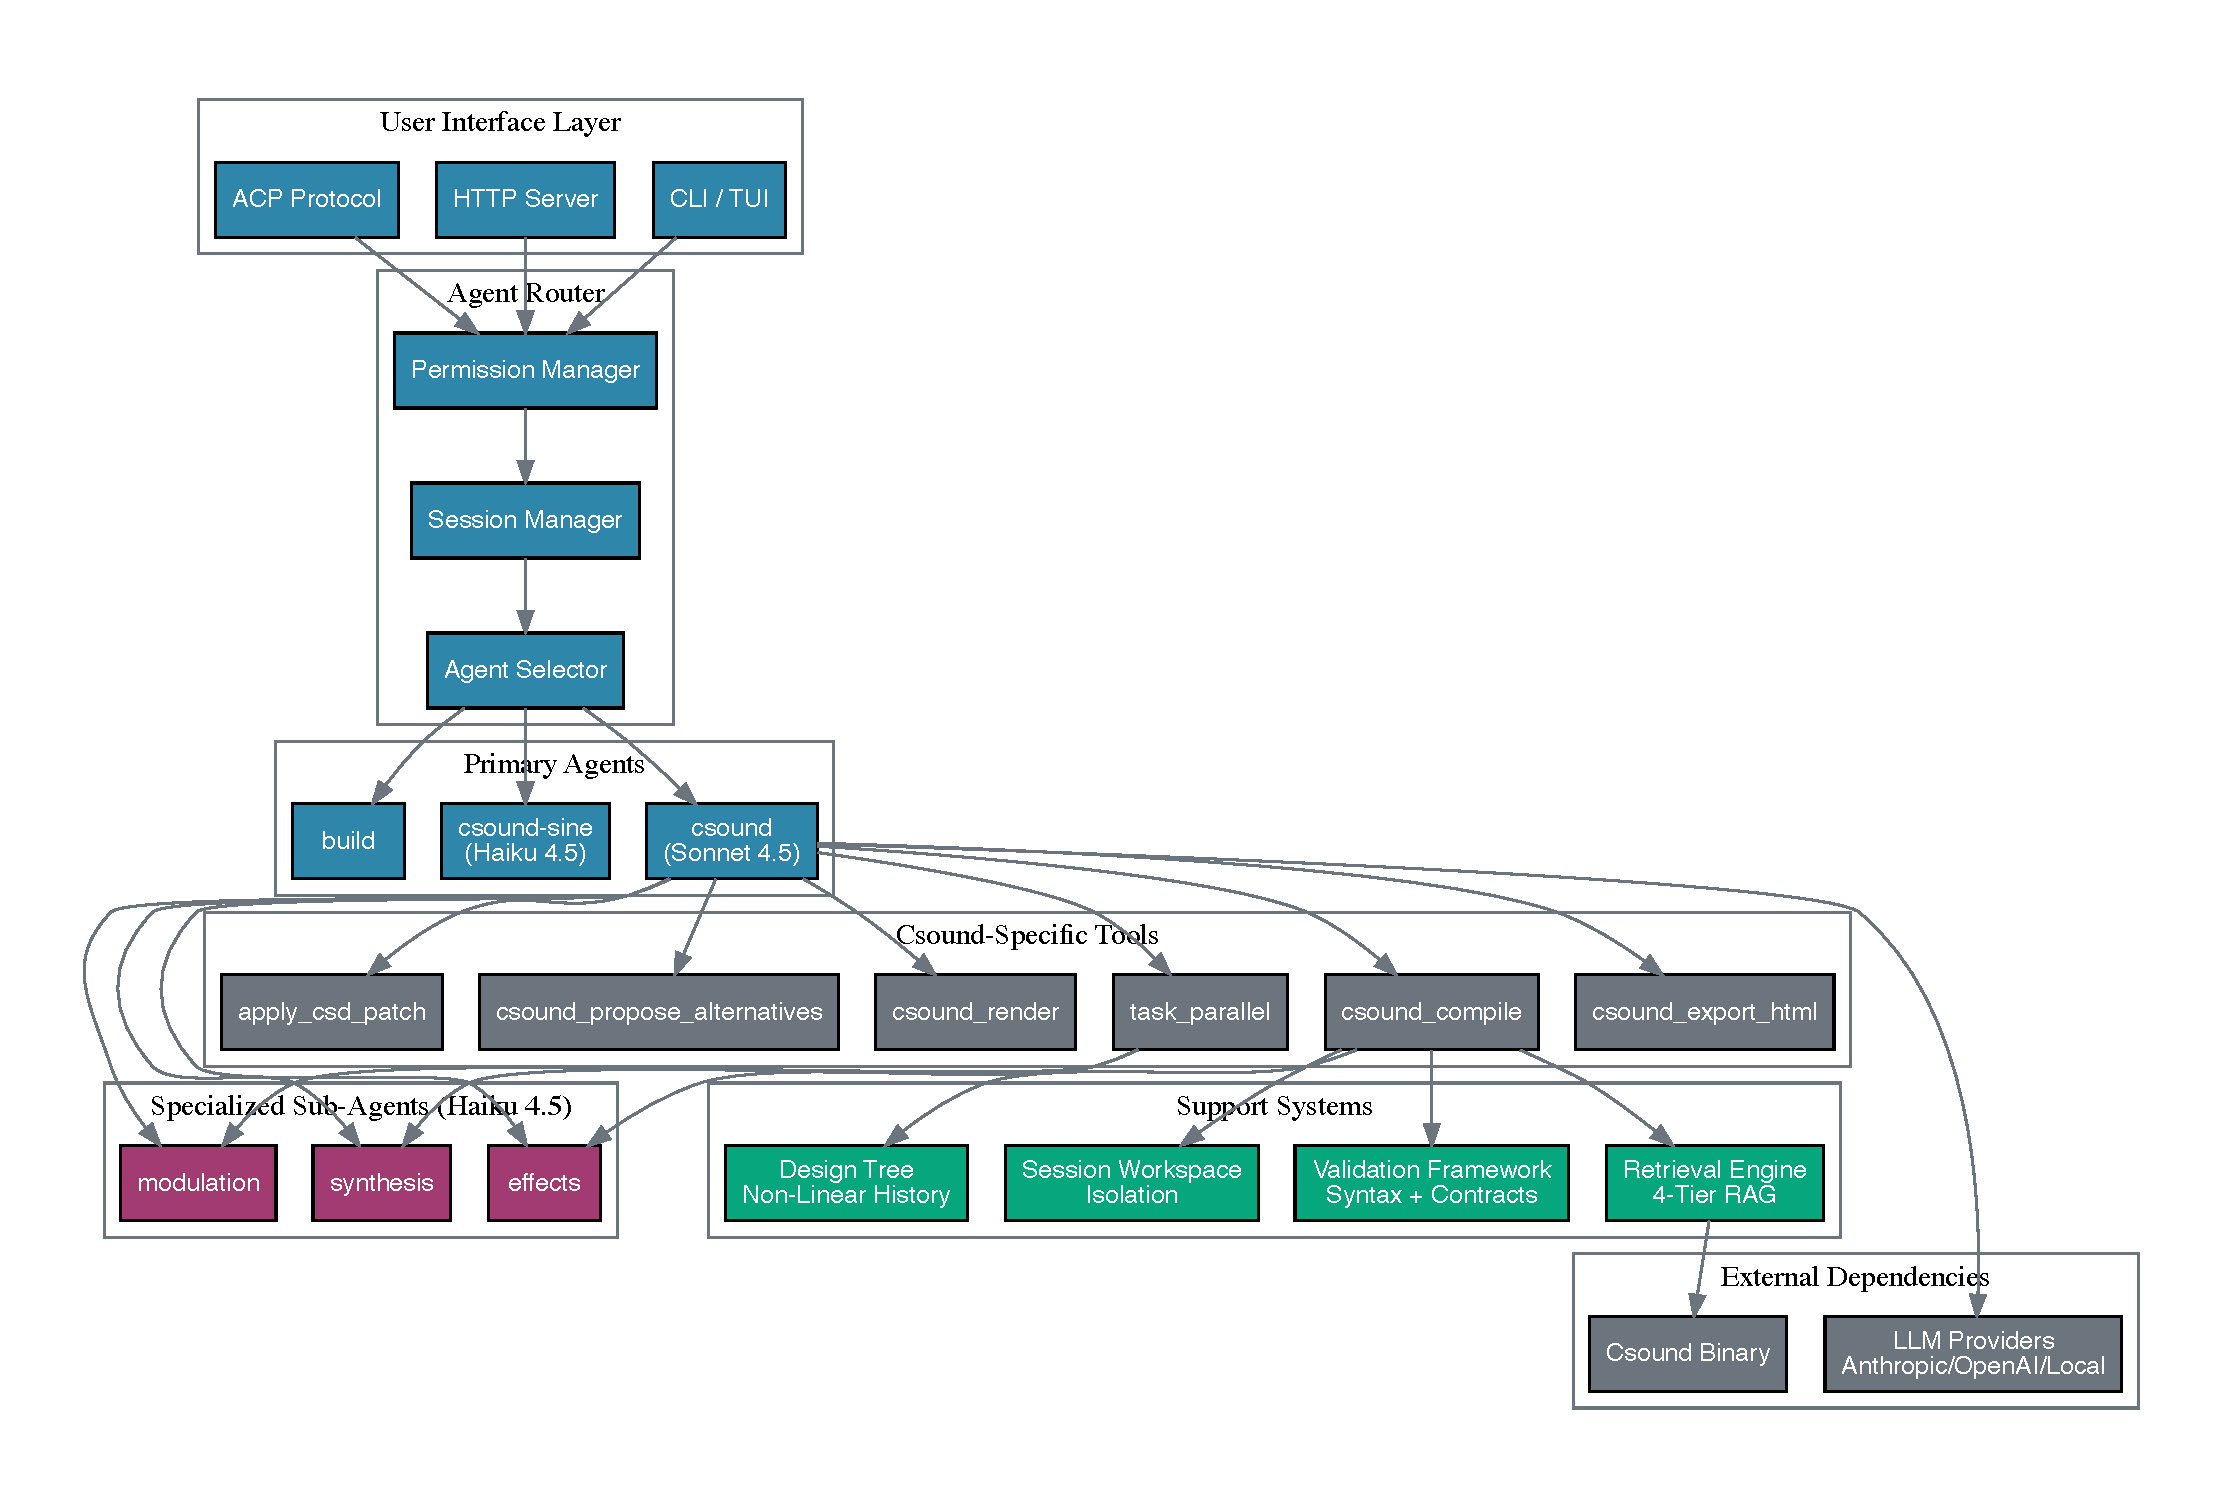
\includegraphics[width=\columnwidth]{figures/architecture-diagram}}
\caption{\label{fig:architecture}{\it Dr.C system architecture showing user interface layer, agent router, primary agents, specialized sub-agents, Csound-specific tools, and support systems including 4-tier RAG, validation framework, session workspace, and design tree.}}
\end{figure}

\subsection{Domain-Specific Tools}

Dr.C extends the base agent framework with Csound-specific tools:

\textbf{csound\_compile:} Syntax validation with structured diagnostics including severity, line/column numbers, error messages, opcode context, error category, and actionable suggestions.

\textbf{csound\_render:} Renders CSD to WAV with configurable duration (default 10s), optional automatic playback, WAV header parsing for metadata, and timeout protection.

\textbf{csound\_propose\_alternatives:} Presents 2--4 alternatives varying by technique, character, complexity. Each includes label, sonic description, approach, and ready-to-apply patch. Creates design tree branch nodes for version control.

\textbf{apply\_csd\_patch:} Structure-aware patching that validates section boundaries (CsInstruments, CsScore, CsOptions, Cabbage), enforces locked parameter constraints, and uses file locking for consistency.

\textbf{csound\_export\_html:} Exports to standalone HTML using @csound/browser CDN with self-contained play/stop controls, code display, and console output.

\textbf{task\_parallel:} Launches 2--4 independent sub-agents in parallel, dramatically reducing latency (e.g., 10s wall-clock vs. 30s sequential for 3 tasks), aggregating results and reporting failures gracefully.

\subsection{Knowledge Retrieval System}

Dr.C implements a four-tier retrieval-augmented generation (RAG) system:

\textbf{Tier 0: Opcode Quick-Reference Cards} — Compact syntax cards for all Csound opcodes with parameters, ranges, common patterns, and pitfalls, domain-tagged for relevance scoring.

\textbf{Tier 1: CSD Example Index} — Indexed working .csd files from CsoundQt examples \cite{csoundqt}, Csound Manual examples \cite{csoundmanual}, FLOSS Manual examples \cite{flossexamples}, Boulanger Csound Instrument Catalog, Cabbage examples \cite{cabbagemanual}, Iain McCurdy Instrument Collection \cite{mccurdycollection}, and Gogins collection \cite{goginscollection}. Metadata searchable via Orama (BM25 + embeddings), full content lazy-loaded on demand, linked to knowledge graph.

\textbf{Tier 2: Prose Knowledge} — Chunked content from \textit{The Csound Book} \cite{boulanger2000csound}, \textit{Csound: A Sound and Music Computing System} \cite{lazzarini2016csound}, Csound 7 reference manual \cite{csoundmanual}, FLOSS Manual \cite{flossmanual}, Csound Journal (all issues) \cite{csoundjournal}, Csound Magazine (all issues) \cite{csoundezine}, Cabbage Manual \cite{cabbagemanual}, and Cabbage Forum \cite{cabbageforum}.

\textbf{Tier 3: Knowledge Graph} — Ontology linking opcodes to synthesis techniques, related opcodes, example CSDs, textbook sections, and acoustic theory.

Query routing uses domain-specific heuristics: technical syntax errors route to Tier 0 (opcode cards), aesthetic requests ("warm reverb") route to Tier 2 (prose), and troubleshooting routes to Tier 1 (working examples).

\section{Alternatives-First Design Paradigm}
\label{sec:alternatives}

Traditional AI assistants generate a single solution, forcing users into a reactive refinement loop. Dr.C introduces an \textbf{alternatives-first} approach where the system proposes multiple design options \textit{before} execution (Figure~\ref{fig:workflow}).

\begin{figure}[t]
\centerline{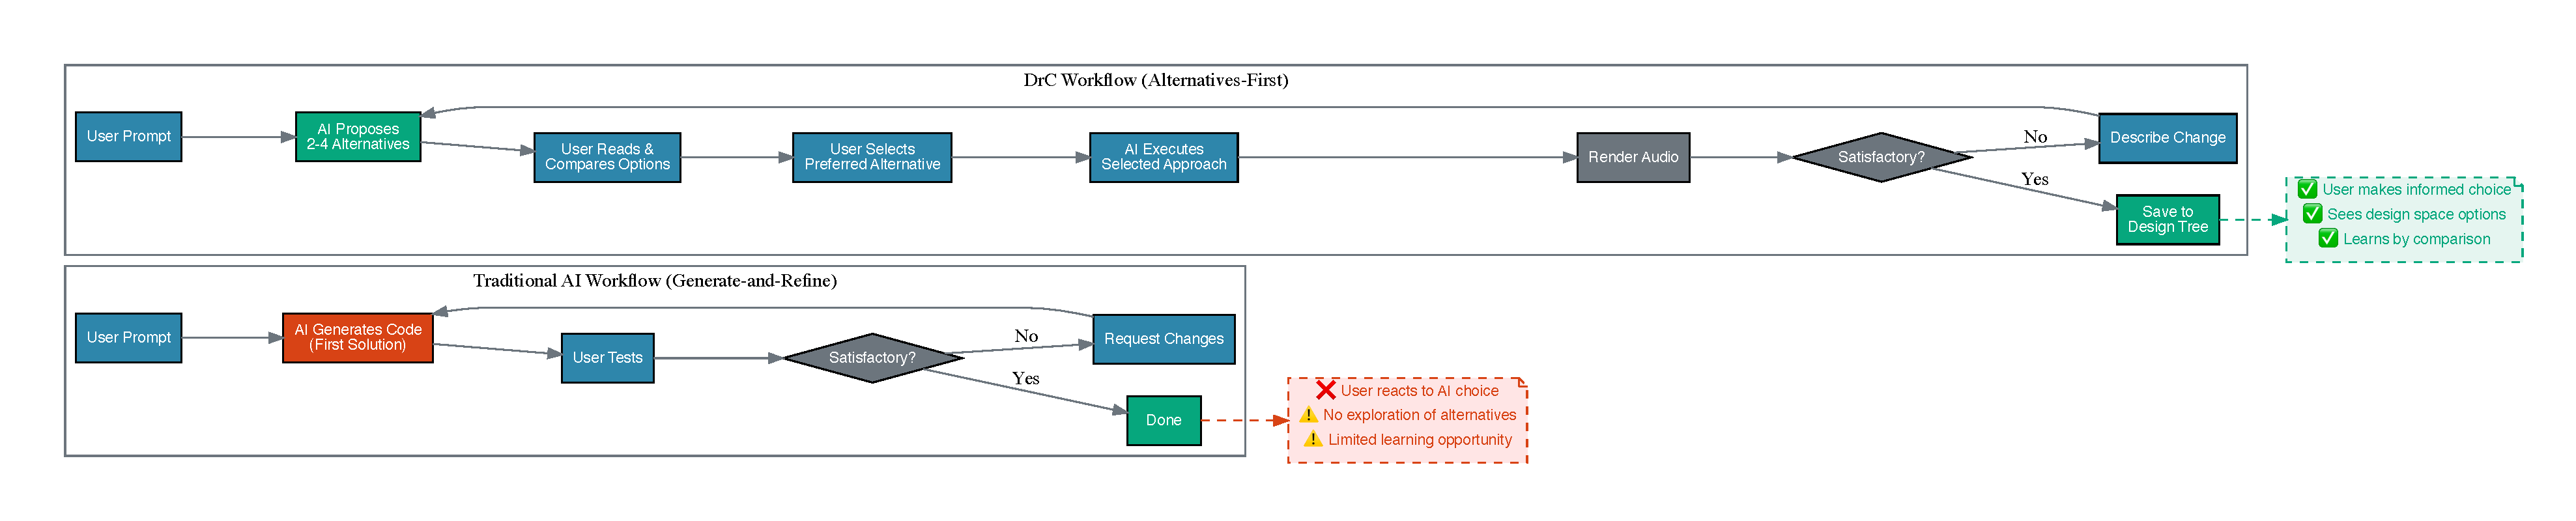
\includegraphics[width=\columnwidth]{figures/alternatives-workflow}}
\caption{\label{fig:workflow}{\it Comparison of traditional AI workflow (generate-and-refine, reactive) versus Dr.C's alternatives-first approach (proactive choice, design space exploration).}}
\end{figure}

\subsection{Design Principles}

\begin{enumerate}
\item \textbf{Proactive Choice:} User selects from alternatives rather than reacting to AI output
\item \textbf{Design Space Exploration:} Alternatives vary along orthogonal dimensions (technique, timbre, complexity)
\item \textbf{Educational Scaffolding:} Each alternative includes technical explanation and parameter semantics
\item \textbf{Creative Agency:} Human maintains control over aesthetic decisions
\end{enumerate}

\subsection{Example Workflow}

User request: \textit{"Add reverb to this synth"}

Dr.C proposes three alternatives:
\begin{enumerate}
\item \textbf{Plate Reverb (Warm, Dense):} Uses \texttt{reverbsc} with long decay, low-pass filtering. Creates smooth, warm spatial image.
\item \textbf{Schroeder Reverb (Bright, Metallic):} Nested allpass filters with short delays. Bright, diffuse character for percussive sources.
\item \textbf{Spring Reverb (Dark, Vintage):} Physical model with resonant modes. Colored, vintage character with boingy artifacts.
\end{enumerate}

Each alternative includes implementation approach, sonic description, and unified diff patch. User selects, system applies and renders immediately.

\section{Semantic Validation Framework}
\label{sec:validation}

Beyond syntax checking, Dr.C implements semantic validation for common error patterns:

\subsection{Cabbage Contract Validation}

Cabbage plugins require strict coupling between UI widgets and instrument code. Dr.C validates:

\begin{itemize}
\item Every \texttt{channel("X")} widget has matching \texttt{chnget "X"} in orchestra
\item All \texttt{chnget} calls use \texttt{port} smoothing to prevent zipper noise
\item Widget ranges match instrument parameter expectations
\item Layout geometry (no overlapping widgets, bounds checking)
\end{itemize}

\subsection{Csound 7 Correctness Rules}

Common AI mistakes from outdated training data:
\begin{itemize}
\item Variable prefix must match opcode output rate (\texttt{aOut = oscili(...)} not \texttt{kOut})
\item Always set \texttt{0dbfs = 1} in orchestra header
\item UDO type strings required in old-style: \texttt{opcode Name, a, ak}
\item Use \texttt{cpsmidinn(noteNum)} to convert MIDI notes, not \texttt{cpsmidi()}
\item \texttt{expseg} values must all be $>$ 0 (use 0.0001 instead of 0)
\item Global audio accumulators must be cleared every k-cycle
\end{itemize}

Validation catches common error categories during development: Cabbage contract violations (mismatched channel declarations), silent output bugs (missing \texttt{out()} calls), Csound 6/7 syntax incompatibilities, and runtime errors (\texttt{expseg} zero values, uncleared accumulators). These checks prevented numerous bugs across the six deployed applications.

\section{Design Tree Exploration}
\label{sec:designtree}

Dr.C captures exploration history as a non-linear design tree (Figure~\ref{fig:designtree}), enabling backtracking, A/B comparison, and documentation of creative process.

\begin{figure}[t]
\centerline{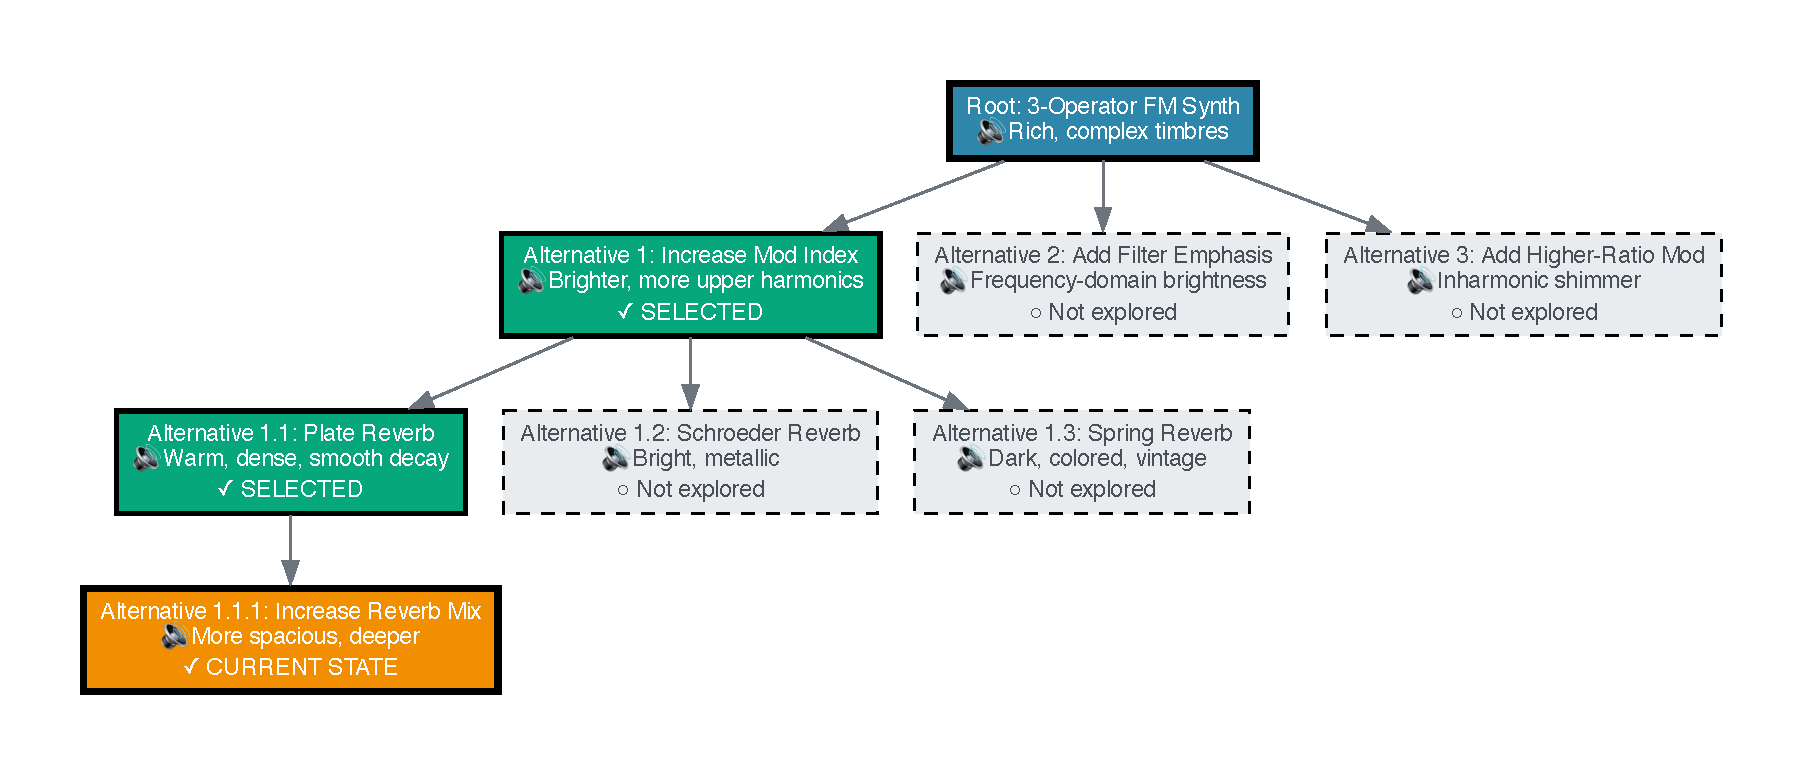
\includegraphics[width=\columnwidth]{figures/design-tree-example}}
\caption{\label{fig:designtree}{\it Design tree showing non-linear exploration of FM synthesis variations. Root node: 3-operator FM synth. Branch 1: modulation index variations. Branch 2: reverb type alternatives. Current state highlighted, unexplored alternatives shown as potential paths.}}
\end{figure}

Each node stores:
\begin{itemize}
\item CSD snapshot hash (efficient deduplication)
\item Sonic characterization metadata ("warm", "bright", "resonant")
\item Alternatives presented (including not-selected branches)
\item User selection reasoning
\item Audio render hash (links to WAV file)
\end{itemize}

Design trees enable pedagogy: students submit trees showing exploration process, not just final code. Instructors assess design thinking, not just implementation.

\section{Educational Deployment}
\label{sec:education}

Dr.C is currently being used in Electronic Production and Design courses at Berklee College of Music—Composition (EP461), DSP (EP413), and Csound (EP337)—as well as in private instruction with high school, undergraduate, and graduate students by both authors. The scope, quality, and quantity of student work using Dr.C is significant, with overwhelmingly positive feedback. Students report that Dr.C's ability to accelerate development enables them to explore more ambitious projects, which increases their motivation to learn synthesis concepts more deeply.

\subsection{Vibe Coding Pedagogy}

"Vibe coding" allows students to describe aesthetic goals ("warm, resonant filter") rather than technical implementation. Dr.C proposes alternatives with technical scaffolding including explanations, parameter meanings, and signal flow diagrams.

\textbf{Block Diagrams:} Dr.C generates ASCII signal flow diagrams demystifying code structure:

\begin{lstlisting}[basicstyle=\ttfamily\tiny]
[Input] -> [FM Osc] -> [Filter] -> [Reverb] -> [Out]
            |            |           |
         [Mod Env]    [Cutoff]   [Decay Time]
\end{lstlisting}

\textbf{From Conception to Production:} Students co-design custom synthesizers and audio processors with Dr.C, then immediately deploy them as audio-reactive web applications or VST/AU plugins using Cabbage. This complete workflow—from aesthetic concept to working production tool—happens within hours. Students create music using instruments and effects they designed themselves, fostering unprecedented ownership, pride, and creative accomplishment. The ability to compose with personally crafted intelligent generative systems transforms the educational experience from passive learning to active tool-building, fundamentally changing how students engage with synthesis and driving creative work to new levels of ambition and sophistication.

\subsection{Educational Outcomes}

Dr.C maintains students as active participants in the collaborative design process—the user-designer remains in the loop at every decision point. Students immediately use their co-designed instruments to create music, play with parameters, explore sonic possibilities, and learn through direct experience. This instant creative feedback loop—design, test, compose—fundamentally transforms the learning experience.

\textbf{Transparency and Learning:} Dr.C teaches while building. All generated code appears directly in the application UI for immediate review, modification, and execution. The design tree preserves complete history, allowing students to retrace any previous step, compare alternatives, and understand evolution of their design. Dr.C generates detailed technical documentation and tutorials explaining parameter meanings, signal flow, and synthesis concepts, enabling students to study and internalize the reasoning behind each design decision.

The alternatives-first approach provides pedagogical scaffolding that helps students understand synthesis concepts while accelerating development workflows. Students can explain the code Dr.C generates and understand the technical reasoning behind design decisions. Because Dr.C generates working, documented, explorable systems instantly, students can focus on creative goals while simultaneously absorbing technical knowledge through guided exploration rather than syntax memorization.

\subsection{Pedagogical Challenges and Curriculum Adaptation}

However, this approach presents significant educational challenges that require careful curriculum design. Students could potentially "push the play button" and let Dr.C generate everything without understanding underlying algorithms, opcodes, or synthesis fundamentals—analogous to a musician who cannot play their instrument. Several critical questions emerge: How do we teach? What do we teach? How do we evaluate learning? How do we measure genuine understanding versus surface-level generation?

\textbf{Foundational Skills First:} Critically, Dr.C is introduced only in the final four weeks of the semester, after students have already established core competencies. Csound students (EP337) have designed basic instruments and effects manually and converted them to plugins via Cabbage. DSP students (EP413) have learned and composed with spectral processing tools \cite{lazzarini2017spectral,roads1996computer,roads2015composing} before building their own with Dr.C. Composition students (EP461) have completed ambient compositions \cite{eno1978ambient,warner2017ambient,pendergrast2003ambient}, Fibonacci-based FM studies, musique concrète projects, and electronic music techniques \cite{chadabe1997electric,cope1997new,cope2001directions,cope2004virtual,norden1969form}, applying principles of algorithmic composition, sound design, and musical form before using AI assistance. This sequencing ensures Dr.C accelerates advanced work rather than replacing foundational learning.

Our current approach includes several safeguards: (1) \textbf{In-class code presentation and defense}, where students must explain their design decisions, justify alternative selections, and demonstrate understanding of signal flow and parameter relationships. (2) \textbf{Design tree documentation}, requiring students to articulate why they chose specific synthesis approaches over alternatives, revealing conceptual understanding. (3) \textbf{Live modification challenges}, where students must debug, modify, or extend their code in real-time without Dr.C assistance, testing foundational knowledge. (4) \textbf{From-scratch assignments}, periodically requiring manual Csound coding to ensure students maintain core technical skills.

The curriculum must balance acceleration with comprehension, ensuring Dr.C scaffolds learning rather than replaces it. Students must demonstrate they can "play the instrument," not merely operate the tool. This requires ongoing pedagogical research, assessment refinement, and honest acknowledgment that AI-assisted education demands new evaluation frameworks that distinguish between tool-assisted creation and foundational mastery.

\textbf{The Paradox of Accessibility:} An ongoing case study with a graduate student—trained in other programming languages and audio tools but new to Csound—reveals a critical question: Does Dr.C motivate users to \textit{learn} Csound deeply, or merely to \textit{use} Csound productively? There exists a possibility that Dr.C could significantly expand Csound adoption while simultaneously reducing the proportion of users who develop deep understanding of synthesis, signal processing, and computer music design principles. Users may create more, accomplish more ambitious projects, yet learn less about underlying fundamentals. This is not necessarily a failure, but rather a fundamental shift in the relationship between tool mastery and creative output that must be recognized, studied longitudinally, and monitored over the coming years. The question remains open: Is a large community of AI-assisted Csound practitioners preferable to a smaller community of synthesis experts? The answer likely depends on educational context, creative goals, and the evolving role of AI in creative practice.

\section{Real-World Deployments}
\label{sec:deployments}

Six applications built with Dr.C, deployed at \url{https://github.com/csounder}:

\begin{enumerate}
\item \textbf{Étude 1:} Generative ambient composition \cite{eno1978ambient} with 14 autonomous instrumental layers and audio-reactive 3D particle visualization
\item \textbf{Weather Sonification:} Maps real-time weather API data to Csound parameters
\item \textbf{Fractal Music Explorer:} L-system grammar \cite{prusinkiewicz1990lsystem} to Csound score generation
\item \textbf{Mandelbrot Explorer:} Mandelbrot set \cite{mandelbrot1983fractal} sonification with zoom navigation
\item \textbf{Memory Maker:} Multimedia slideshow creator for music therapy combining photos, videos, and music. Version 2 will add sing-along features with pitch correction via Csound's phase vocoder opcodes
\item \textbf{Csound Drum Machine:} Pattern and arrangement sequencer allowing users to string together patterns and sub-patterns into complete songs. Features customizable drum kits with individual timbre, envelope, and balance controls per sound, plus effects including resonators, ring modulators, and multi-tap delays
\end{enumerate}

Dr.C facilitated the creation, customization, and modification of these applications in hours and days rather than weeks and months. Applications are being deployed in Berklee courses and demonstrate Dr.C's ability to scaffold complex generative systems, algorithmic composition, therapeutic applications, and rhythm programming. Figures~\ref{fig:etude1}--\ref{fig:drummachine} show screenshots of selected deployed applications.

\begin{figure}[t]
\centerline{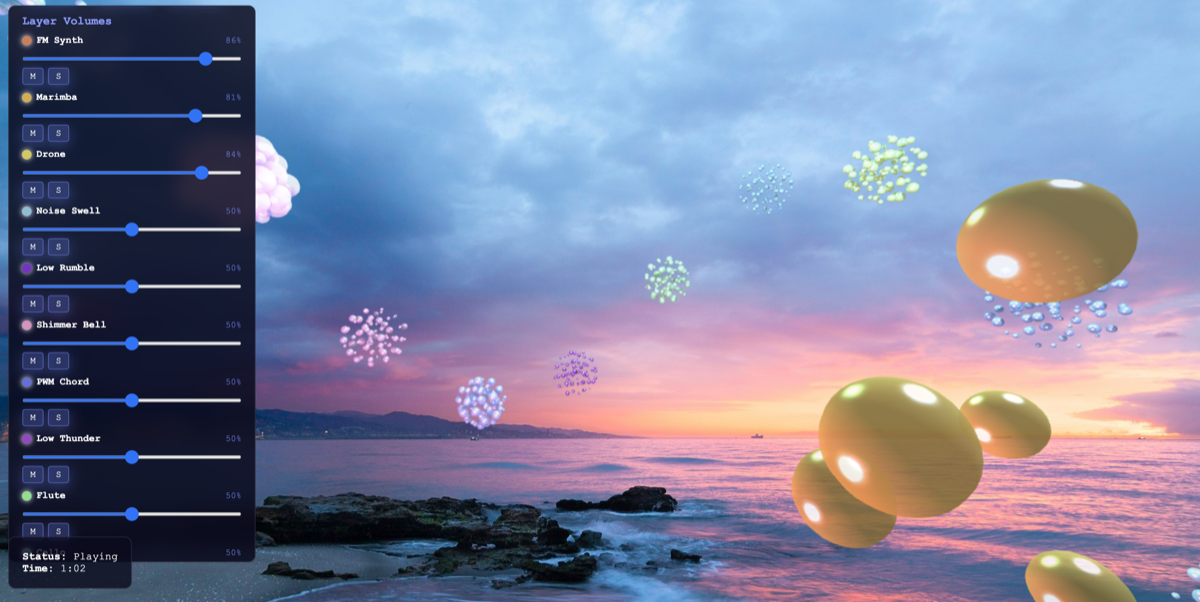
\includegraphics[width=\columnwidth]{figures/etude1-screenshot}}
\caption{\label{fig:etude1}{\it Étude 1: Generative ambient composition with 14 autonomous instrumental layers (left panel) and audio-reactive 3D particle visualization responding to live audio levels.}}
\end{figure}

\begin{figure}[t]
\centerline{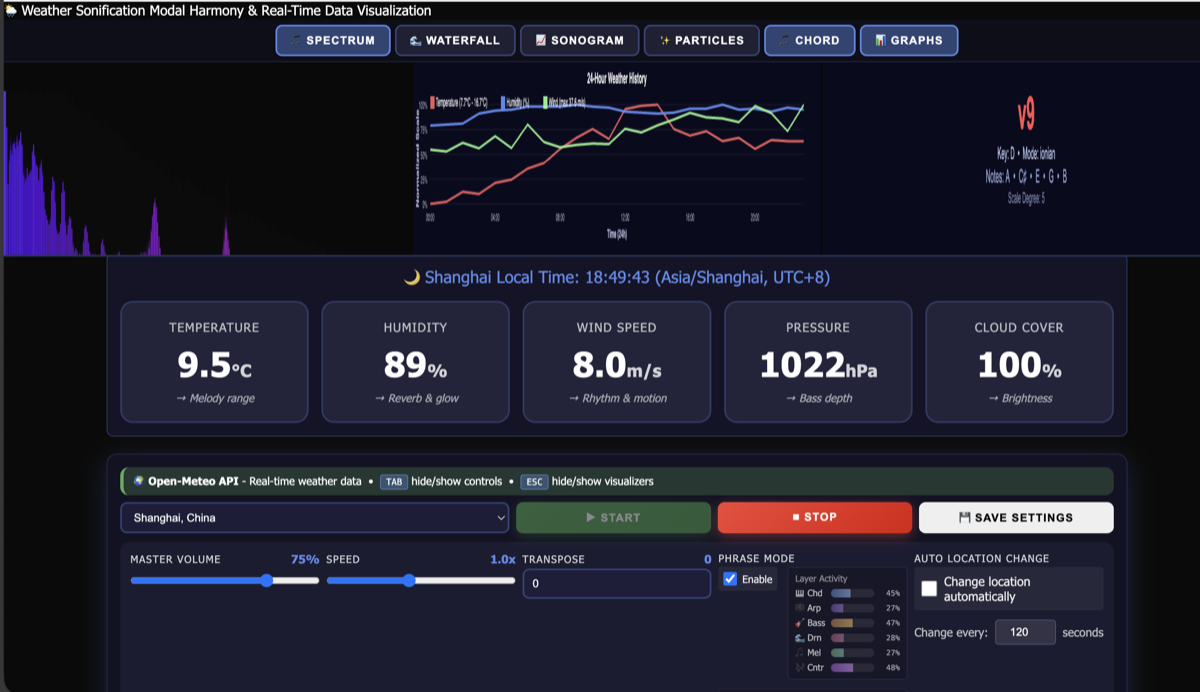
\includegraphics[width=\columnwidth]{figures/weather-screenshot}}
\caption{\label{fig:weather}{\it Weather Sonification: Real-time weather API data mapped to Csound synthesis parameters including temperature, pressure, wind speed, and humidity.}}
\end{figure}

\begin{figure}[t]
\centerline{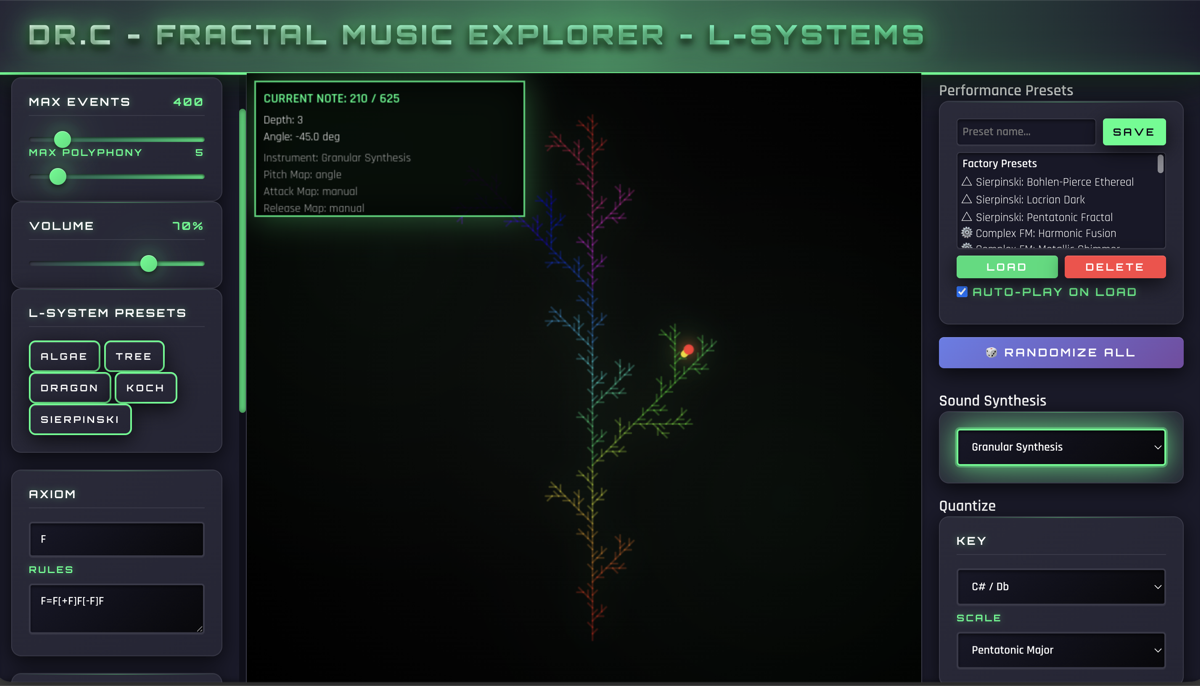
\includegraphics[width=\columnwidth]{figures/fractal-screenshot}}
\caption{\label{fig:fractal}{\it Fractal Music Explorer: L-system grammar editor with visual growth animation and symbol-to-pitch mapping for algorithmic composition.}}
\end{figure}

\begin{figure}[t]
\centerline{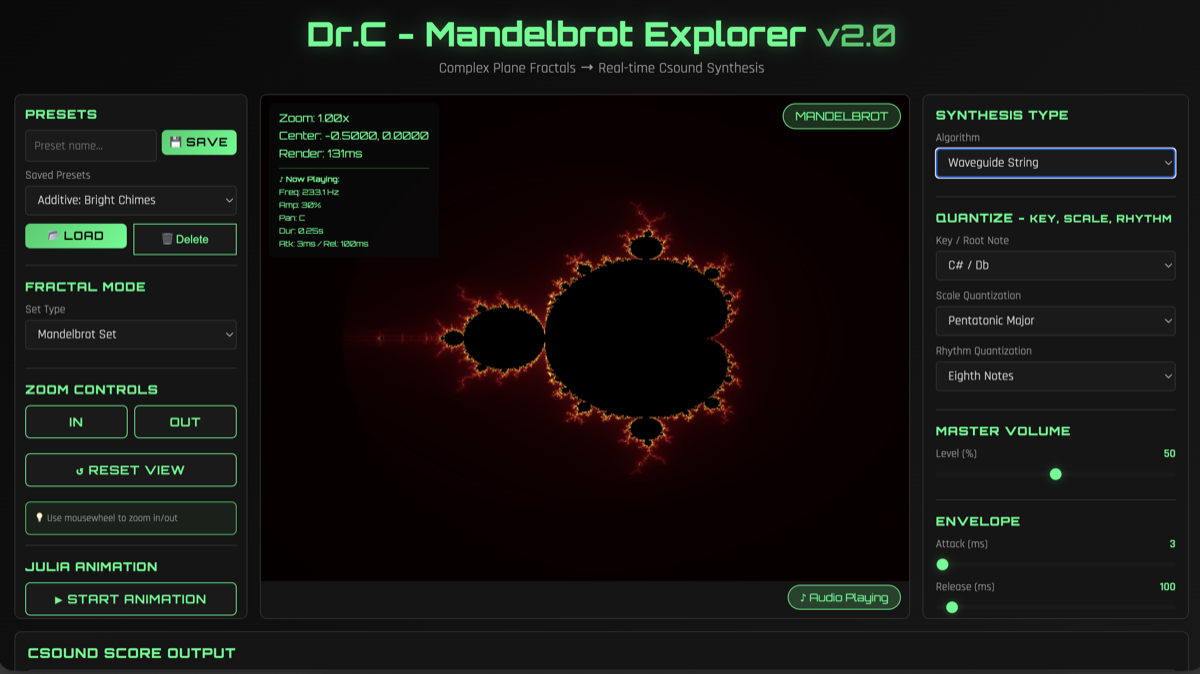
\includegraphics[width=\columnwidth]{figures/mandelbrotexplorer}}
\caption{\label{fig:mandelbrot}{\it Mandelbrot Explorer: Interactive fractal sonification with zoom navigation and coordinate-to-synthesis parameter mapping.}}
\end{figure}

\begin{figure}[t]
\centerline{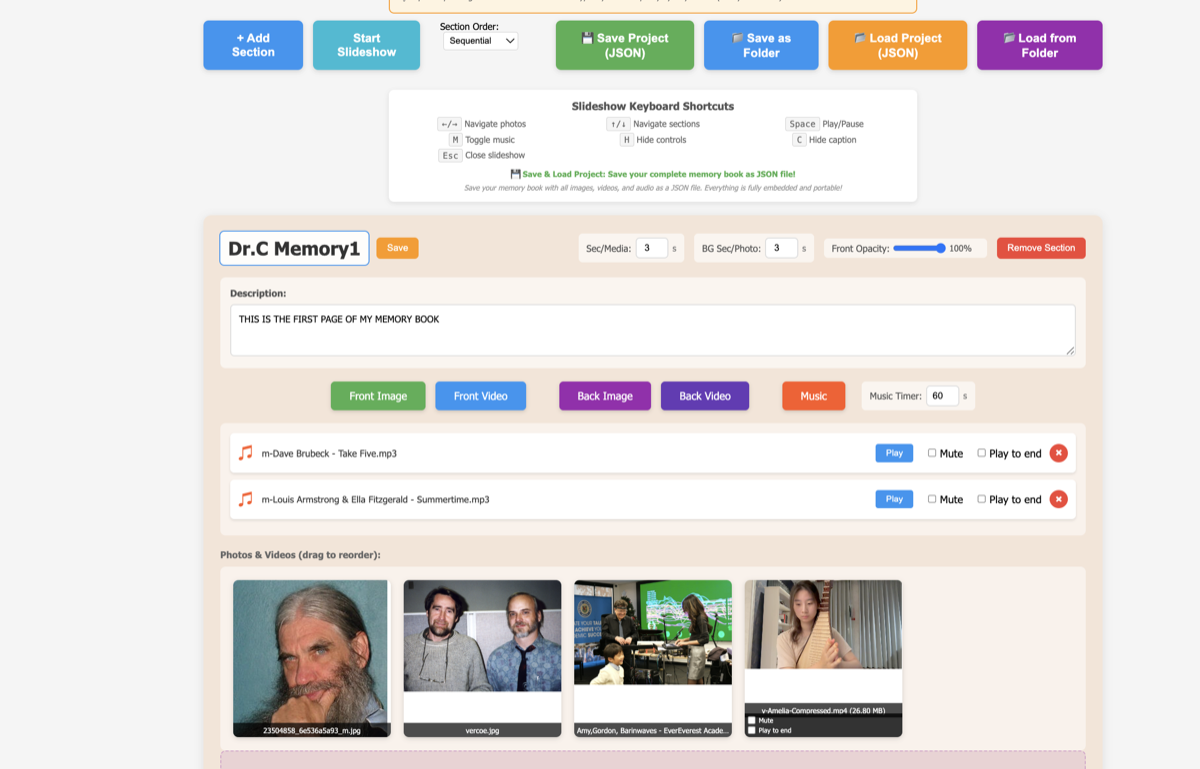
\includegraphics[width=\columnwidth]{figures/memorymaker-screenshot}}
\caption{\label{fig:memorymaker}{\it Memory Maker: Multimedia slideshow creator for music therapy combining photos, videos, and musical playback with automatic transitions.}}
\end{figure}

\begin{figure}[t]
\centerline{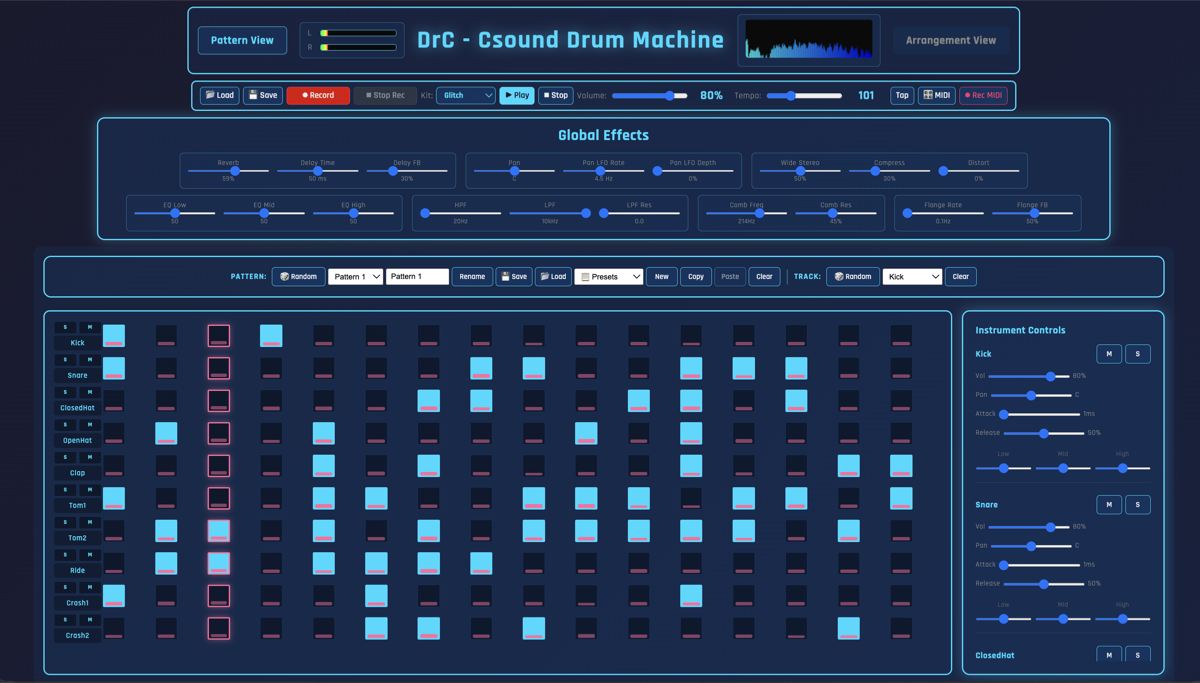
\includegraphics[width=\columnwidth]{figures/drummachine-screenshot}}
\caption{\label{fig:drummachine}{\it Csound Drum Machine: Pattern and arrangement sequencer with customizable drum kits, comprehensive effects processing, and song structure builder.}}
\end{figure}

\section{Ethical Considerations}
\label{sec:ethics}

\subsection{Author-as-Curator Model}

Dr.C's knowledge base is curated from the authors' published works and expert-selected community resources including \textit{The Csound Book} \cite{boulanger2000csound}, foundational texts on spectral processing \cite{lazzarini2017spectral}, computer music \cite{roads1996computer,roads2015composing}, electronic music history \cite{chadabe1997electric}, ambient composition \cite{eno1978ambient,warner2017ambient,pendergrast2003ambient}, composition techniques \cite{cope1997new,cope2001directions,cope2004virtual}, and musical form \cite{norden1969form}, plus the Classic Boulanger Csound Instrument Catalog, Amsterdam Catalog \cite{amsterdamcatalog}, FLOSS Manual \cite{flossmanual} and examples \cite{flossexamples}, Csound Journal \cite{csoundjournal}, Csound Magazine \cite{csoundezine}, Cabbage Manual \cite{cabbagemanual} and forum \cite{cabbageforum}, CsoundQt manual and examples \cite{csoundqt}, and the Iain McCurdy Instrument Collection \cite{mccurdycollection} and Gogins collection \cite{goginscollection}. This "author-as-curator" model ensures:

\begin{itemize}
\item Explicit consent (author controls training data)
\item Attribution preserved in retrieval
\item Educational intent primary
\item No corporate web scraping
\end{itemize}

\subsection{Open Source Commitment}

Dr.C is MIT-licensed, works with local models (Ollama), and designed for FLOSS ecosystem integration. All deployed applications are open-source with full CSD code visible.

\subsection{Human Agency}

Alternatives-first design ensures humans remain in creative control. Dr.C is a \textit{collaborator}, not autonomous generator. Design trees document human decision-making, not just AI output.

\section{Related Work}
\label{sec:related}

\textbf{AI-Assisted Programming:} GitHub Copilot, Cursor, and Replit Agent provide general-purpose code completion but lack domain specialization, semantic validation, and alternatives-first interaction.

\textbf{Music AI Systems:} Magenta, AIVA, and MuseNet generate musical content but do not scaffold \textit{learning} or provide \textit{tool-level} assistance for synthesis programming.

\textbf{Csound Education:} CsoundQt \cite{csoundqt}, Web-Csound, and Cabbage provide IDEs but no intelligent assistance. Blue's pattern language offers abstraction but not AI collaboration.

Dr.C uniquely combines domain-specialized AI with educational scaffolding and FLOSS principles.

\section{Future Work}
\label{sec:future}

Ten additional applications are in development: Strange Attractor Explorer (chaos sonification), Game of Life Music Maker (cellular automata), DNA Music Machine (genetic sequences), Sacred Tones Explorer (therapeutic frequencies), My Electronic Poème \cite{varese1958poeme} (ambisonic spatial audio), Fibonacci FM Composer \cite{chowning1977stria} (golden ratio synthesis), CsoundRave \cite{bt2005binary} (generative EDM), Csound Cross Synthesizer (live cross-synthesis), Csound Morpher (spectral morphing), and Csound Spectral Mutator (spectral transformation). All will be browser-based tools and freely available under MIT license.

We are also integrating the Csound Reference Manual and FLOSS Manual into Dr.C's knowledge retrieval for real-time opcode documentation and working examples during the design process.

\section{Conclusion}
\label{sec:conclusion}

Dr.C demonstrates that domain-specialized AI assistants can significantly outperform general-purpose tools for creative technical work in FLOSS audio. The alternatives-first paradigm, multi-tier knowledge retrieval, semantic validation, and design tree exploration represent transferable patterns for other specialized domains.

Educational deployment shows Dr.C scaffolds conceptual understanding while accelerating development workflows, though with trade-offs in manual proficiency. The author-as-curator model provides an ethical template for consent-based AI training.

Dr.C is freely available under MIT license, representing a community resource for Csound education and a reference implementation for domain-specialized AI in FLOSS audio development.

\section{Acknowledgments}

The authors thank Berklee students for feedback and the Csound community for their contributions. Special thanks to Victor Lazzarini, Joachim Heintz, Iain McCurdy (whose extensive instrument collection has been foundational and incredibly inspiring), Steven Yi, Hlödver Sigurdsson, Rory Walsh, Tarmo Johannes, and Michael Gogins whose reference materials, tutorials, and models form Dr.C's knowledge base.

\begin{thebibliography}{9}

\bibitem{boulanger2000csound}
R. Boulanger, Ed., \textit{The Csound Book: Perspectives in Software Synthesis, Sound Design, Signal Processing, and Programming}. MIT Press, 2000.

\bibitem{lazzarini2016csound}
V. Lazzarini, S. Yi, J. Heintz, Ø. Brandtsegg, and I. McCurdy, \textit{Csound: A Sound and Music Computing System}. Springer, 2016.

\bibitem{lazzarini2017spectral}
V. Lazzarini, \textit{Spectral Music Design: A Computational Approach}. Oxford University Press, 2017.

\bibitem{roads1996computer}
C. Roads, \textit{The Computer Music Tutorial}. MIT Press, 1996.

\bibitem{roads2015composing}
C. Roads, \textit{Composing Electronic Music: A New Aesthetic}. Oxford University Press, 2015.

\bibitem{chadabe1997electric}
J. Chadabe, \textit{Electric Sound: The Past and Promise of Electronic Music}. Prentice Hall, 1997.

\bibitem{cope1997new}
D. Cope, \textit{Techniques of the Contemporary Composer}. Schirmer Books, 1997.

\bibitem{cope2001directions}
D. Cope, \textit{New Directions in Music}. Waveland Press, 2001.

\bibitem{cope2004virtual}
D. Cope, \textit{Virtual Music: Computer Synthesis of Musical Style}. MIT Press, 2004.

\bibitem{norden1969form}
H. Norden, \textit{Form: The Silent Language}. Crescendo Publishing, 1969.

\bibitem{warner2017ambient}
D. Warner, \textit{Composing Ambient Music: Inspirational Strategies for Creating Ambient Electronic Music}. Self-published, 2017.

\bibitem{pendergrast2003ambient}
M. Pendergrast, \textit{The Ambient Century: From Mahler to Trance---The Evolution of Sound in the Electronic Age}. Bloomsbury, 2003.

\bibitem{csoundwebsite}
"Csound — A Sound and Music Computing System," \url{https://csound.com/}, accessed March 2026.

\bibitem{csoundmanual}
"The Csound Reference Manual," \url{https://csound.com/docs/manual/index.html}, accessed March 2026.

\bibitem{flossmanual}
J. Heintz, A. Hofmann, and I. McCurdy, "FLOSS Manual — Csound," \url{https://flossmanual.csound.com/}, accessed March 2026.

\bibitem{flossexamples}
"FLOSS Manual Csound Examples," \url{https://github.com/csudo/csudo.github.io}, accessed March 2026.

\bibitem{amsterdamcatalog}
"The Amsterdam Catalog of Csound Computer Instruments," \url{http://www.codemist.co.uk/AmsterdamCatalog/}, accessed March 2026.

\bibitem{goginscollection}
M. Gogins, "Extended Csound and Web Audio Examples," \url{https://michaelgogins.tumblr.com/}, accessed March 2026.

\bibitem{cabbagemanual}
R. Walsh, "Cabbage Audio — Documentation and Examples," \url{https://cabbageaudio.com/docs/}, accessed March 2026.

\bibitem{cabbageforum}
"Cabbage Audio Forum," \url{https://forum.cabbageaudio.com/}, accessed March 2026.

\bibitem{csoundjournal}
"The Csound Journal," \url{https://csoundjournal.com/}, accessed March 2026.

\bibitem{csoundezine}
"The Csound Magazine," \url{http://www.csounds.com/ezine/}, accessed March 2026.

\bibitem{mccurdycollection}
I. McCurdy, "Iain McCurdy Csound Instrument Collection," \url{http://iainmccurdy.org/csound.html}, accessed March 2026.

\bibitem{csoundqt}
A. Cabrera, "CsoundQt Examples," \url{https://github.com/CsoundQt/CsoundQt/tree/develop/src/Examples}, accessed March 2026.

\bibitem{mandelbrot1983fractal}
B. Mandelbrot, \textit{The Fractal Geometry of Nature}. W. H. Freeman, 1983.

\bibitem{prusinkiewicz1990lsystem}
P. Prusinkiewicz and A. Lindenmayer, \textit{The Algorithmic Beauty of Plants}. Springer-Verlag, 1990.

\bibitem{varese1958poeme}
E. Varèse, \textit{Poème électronique}. Philips Pavilion, Brussels World's Fair, 1958.

\bibitem{chowning1977stria}
J. Chowning, \textit{Stria}. Stanford University, 1977.

\bibitem{eno1978ambient}
B. Eno, \textit{Ambient 1: Music for Airports}. Polydor Records, 1978.

\bibitem{mccurdy2012haiku}
I. McCurdy, \textit{Csound Haiku}. Self-published collection, 2012.

\bibitem{bt2005binary}
BT (Brian Transeau), \textit{This Binary Universe}. Nettwerk Records, 2005.

\end{thebibliography}

\end{document}
